\section{Homepage}

A website homepage is the equivalent of a shop window. The goal of the 
homepage is to introduce the user and present essential information as 
effectively as possible. In fact, the homepage must take into account the 
identity of the person it represents (in this case the company), the 
navigation, the speed of presentation of the contents and tools 
(for example, the search bar).

\subsection{6W}

For the purpose of evaluating how the information is presented, the site 
will be analyzed following the 6 axes: \textit{Where}, \textit{Who}, 
\textit{Why}, \textit{What}, \textit{When}, \textit{How}. 

\subsubsection{Where}

\centerline{\textit{Which site did I arrive at? What kind of content does 
the website offer me?}}
At first glance, it is possible to notice a slogan that allows the user 
to directly understand the theme the company deals with 
(fig. \ref{fig:homepage-1}). Furthermore, it is also possible to see at 
first glance that the company develops a product that can be used via 
mobile devices. It is also possible to notice the sentence placed under 
the slogan, in which it is explained what is the product that the company 
develops.

\begin{figure}[H]
	\centering
	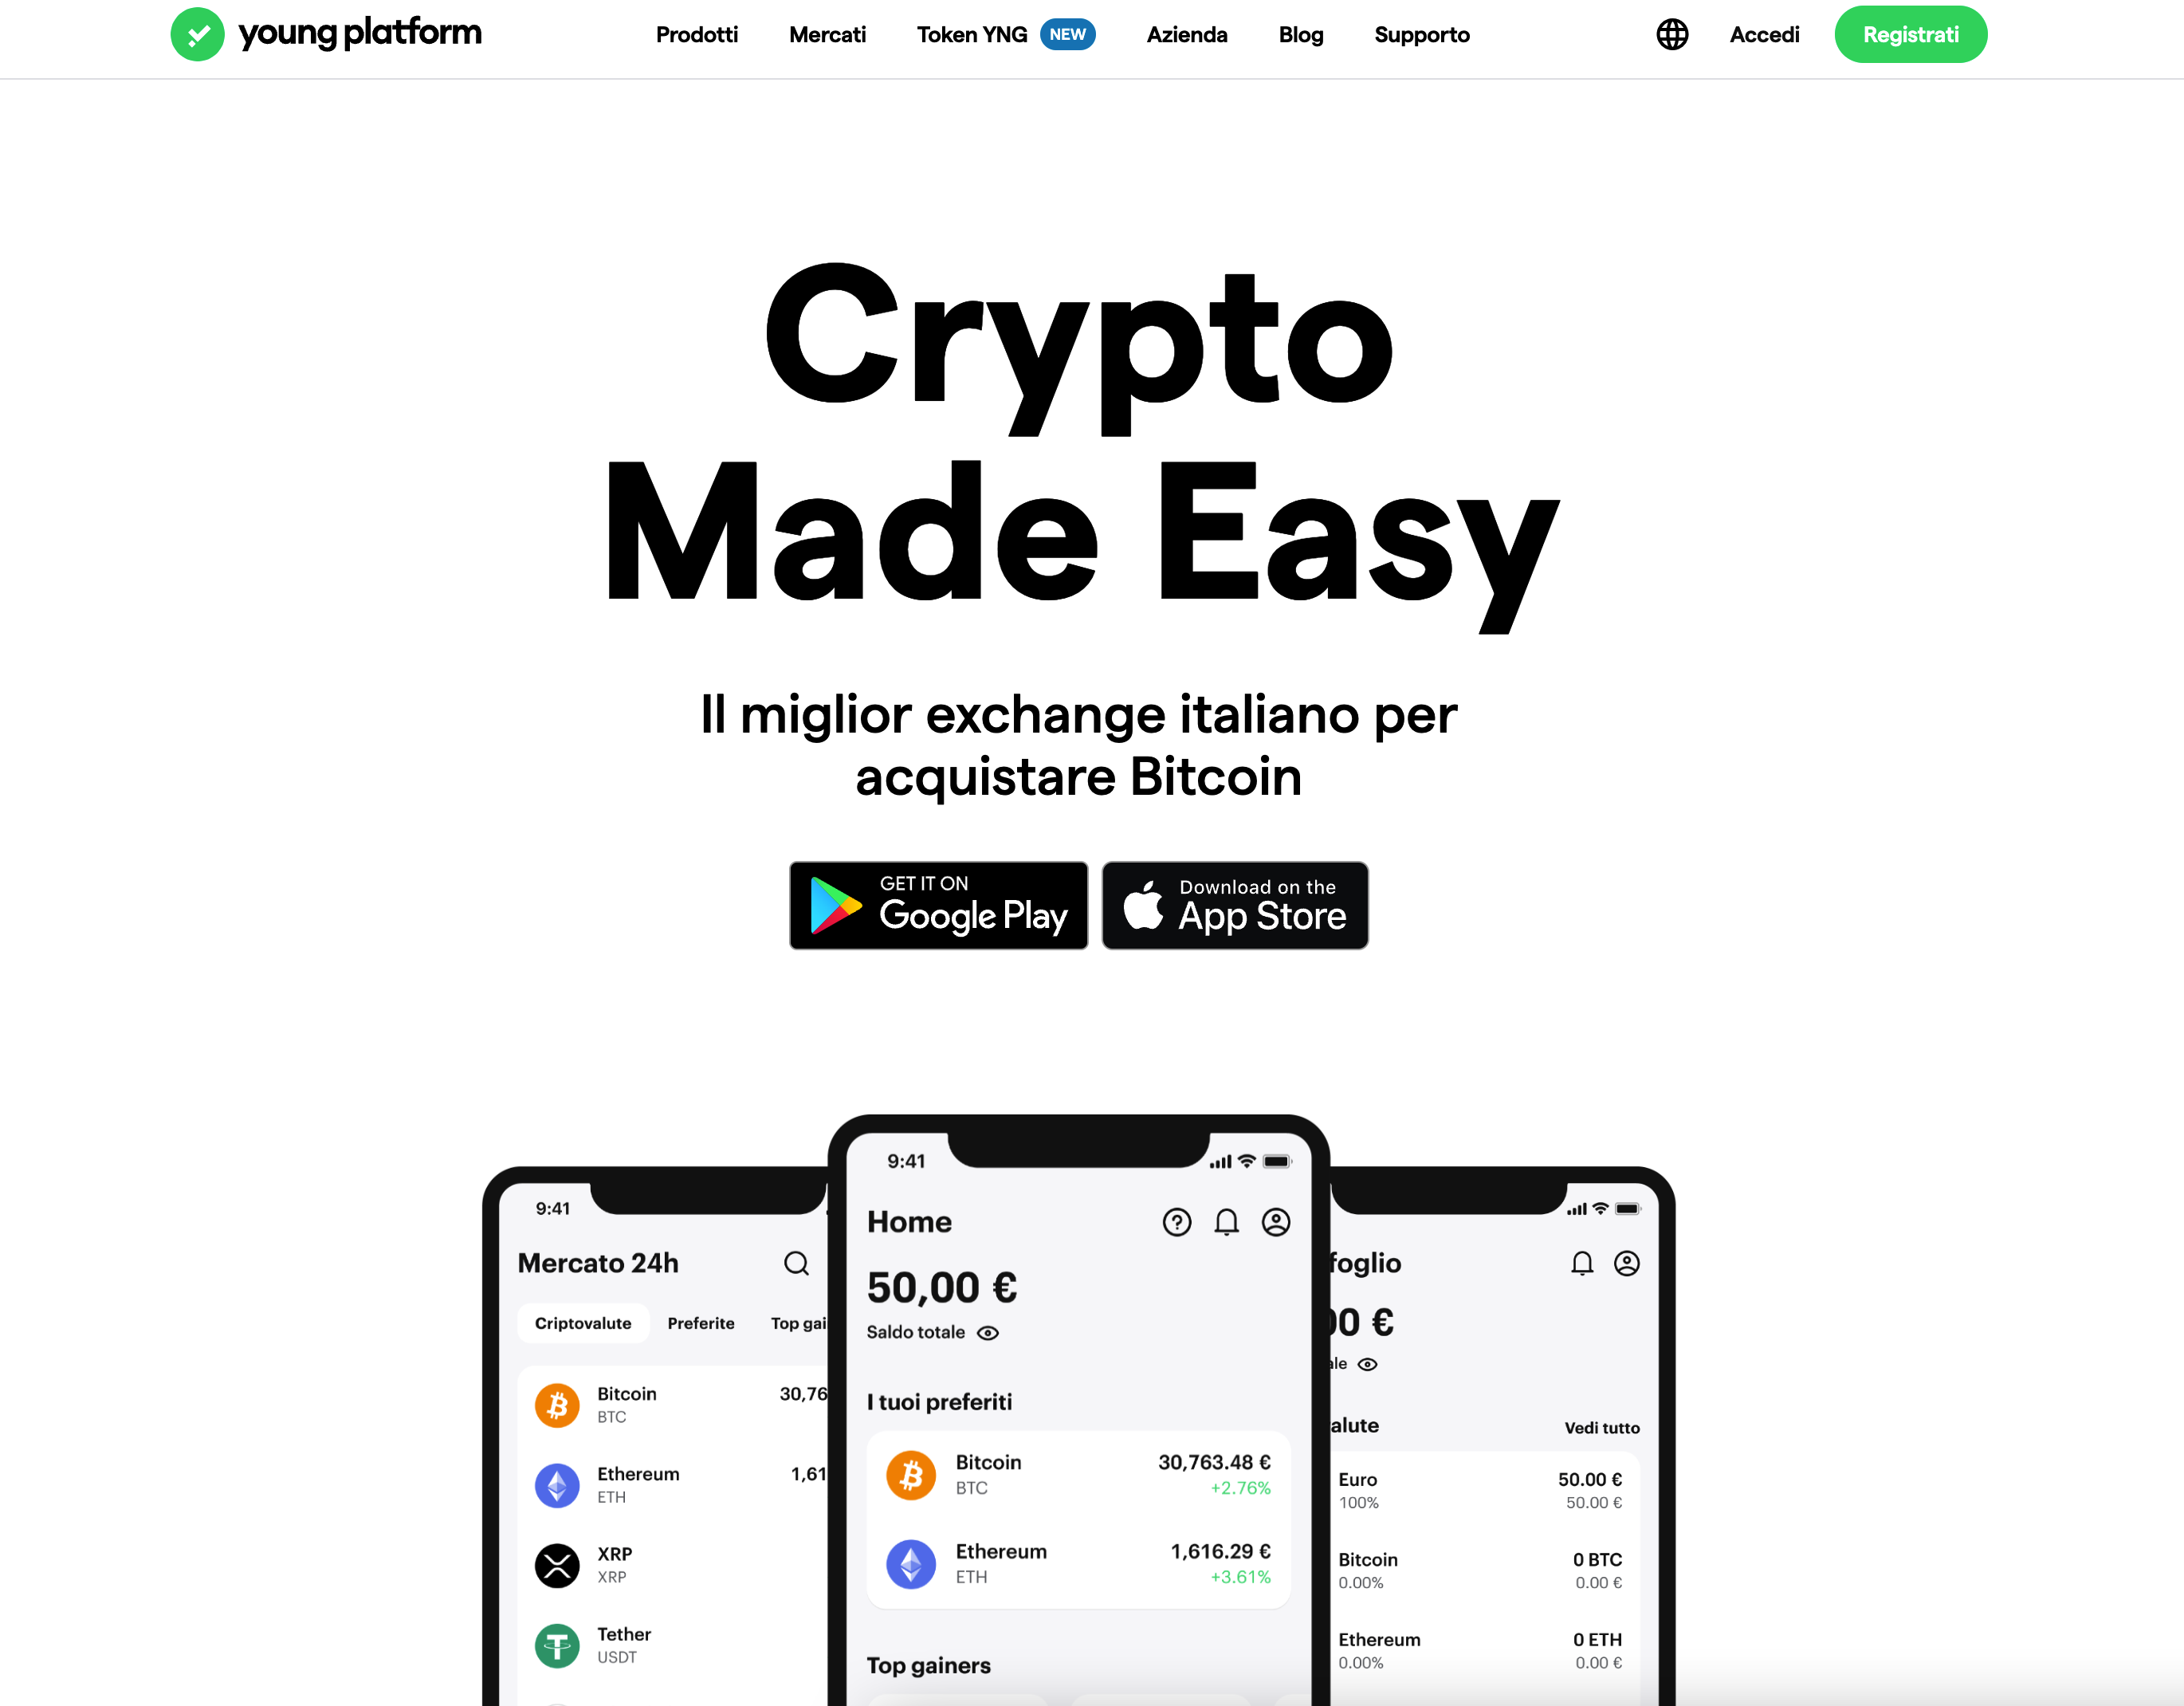
\includegraphics[width=0.80\textwidth]{res/images/homepage-1.png}
	\caption{First section of the homepage.}
	\label{fig:homepage-1}
\end{figure}

\subsubsection{Who}

\centerline{\textit{Who is behind this site?}}
At first glance it is not possible to understand who is behind this site. 
As mentioned above, the name of the website does not allow any information 
to be drawn to be able to guess who could be behind the creation of the 
site. In the menu at the top center, you can see the \textit{Azienda} 
(\textit{Company}) item and from there a menu opens in which the 
\textit{Parlano di noi} (\textit{They talk about us}) item is 
present (fig. \ref{fig:who-we-are-1}). By clicking on this item, you are 
redirected to a page that collects a series of articles about the company 
(fig. \ref{fig:who-we-are-2}). So, at first glance it is not easy to 
understand who is the team behind the site and consequently who made 
these products. To get additional information about the company it is 
therefore necessary to carry out a preliminary research. From the 
user's point of view, this represents a big disadvantage and could be a 
reason not to continue viewing the website.

\begin{figure}[H]
	\centering
	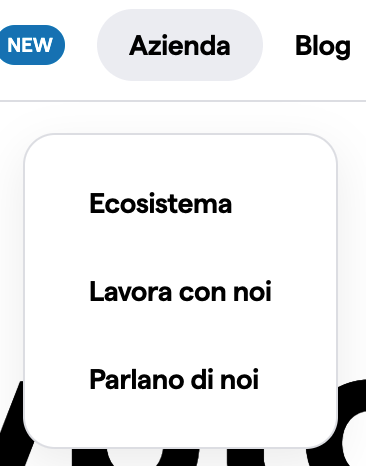
\includegraphics[width=0.30\textwidth]{res/images/who-we-are-1.png}
	\caption{Main menu - \textit{Parlano di noi} (\textit{They talk about us}).}
	\label{fig:who-we-are-1}
\end{figure}

\begin{figure}[H]
	\centering
	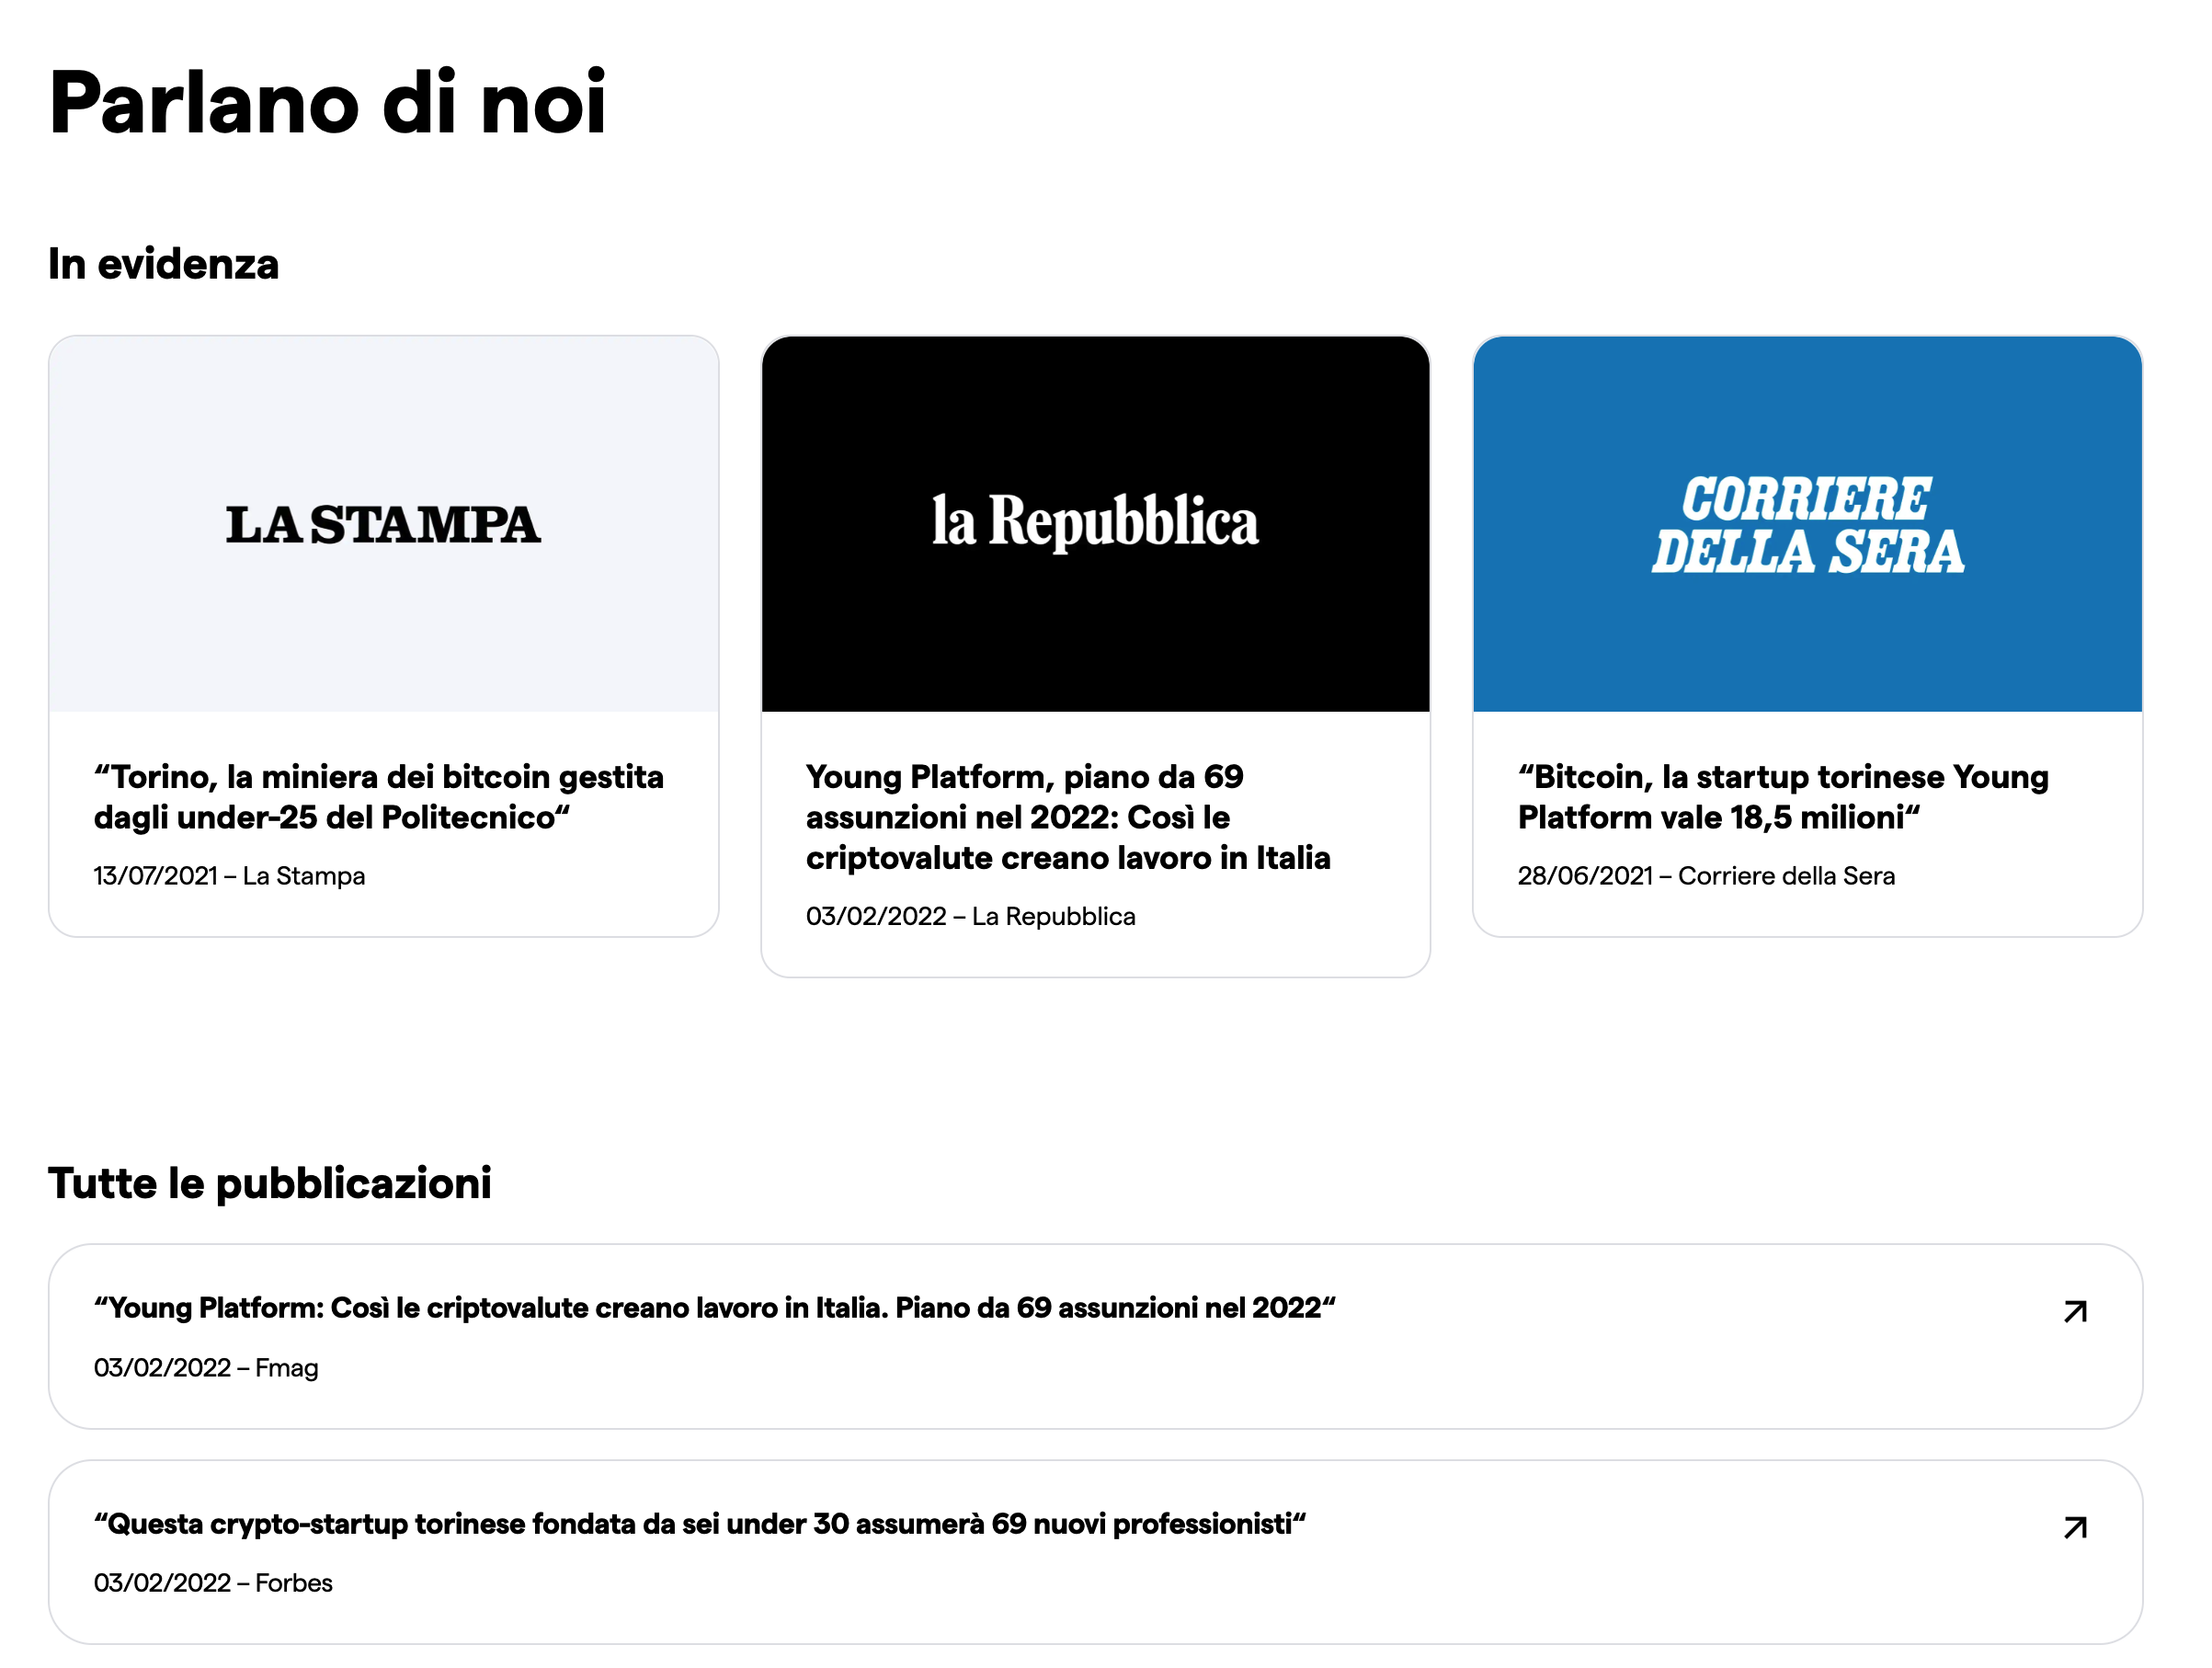
\includegraphics[width=0.80\textwidth]{res/images/who-we-are-2.png}
	\caption{\textit{Parlano di noi} (\textit{They talk about us}) page.}
	\label{fig:who-we-are-2}
\end{figure}

\newpage

\subsubsection{Why}

\centerline{\textit{Why should the user stay on the site? What advantages 
does it offer?}}
The aim of the site is to mainly attract the attention of those new users 
who want to enter this world. Therefore, the user (in particular, a novice 
user) is encouraged to stay on the site, as it can learn a lot of 
information: from the technological foundations on which cryptocurrencies are 
based to the latest industry news. For a more experienced user in the 
industry, this site may not be attractive from their point of view, as the 
site mainly features content and products aimed at beginners. The company 
has also developed a product dedicated to expert users, but the homepage 
does not mention this product except in the footer, under 
\textit{Young Platform Pro} (second item in the first column on the left, 
fig. \ref{fig:footer}). However, it must be remembered that the company's 
goal is to introduce the largest number of novice users to this industry. 
So, I suppose that an inexperienced user is very interested in the contents 
of the homepage and can benefit from it.

\begin{figure}[H]
	\centering
	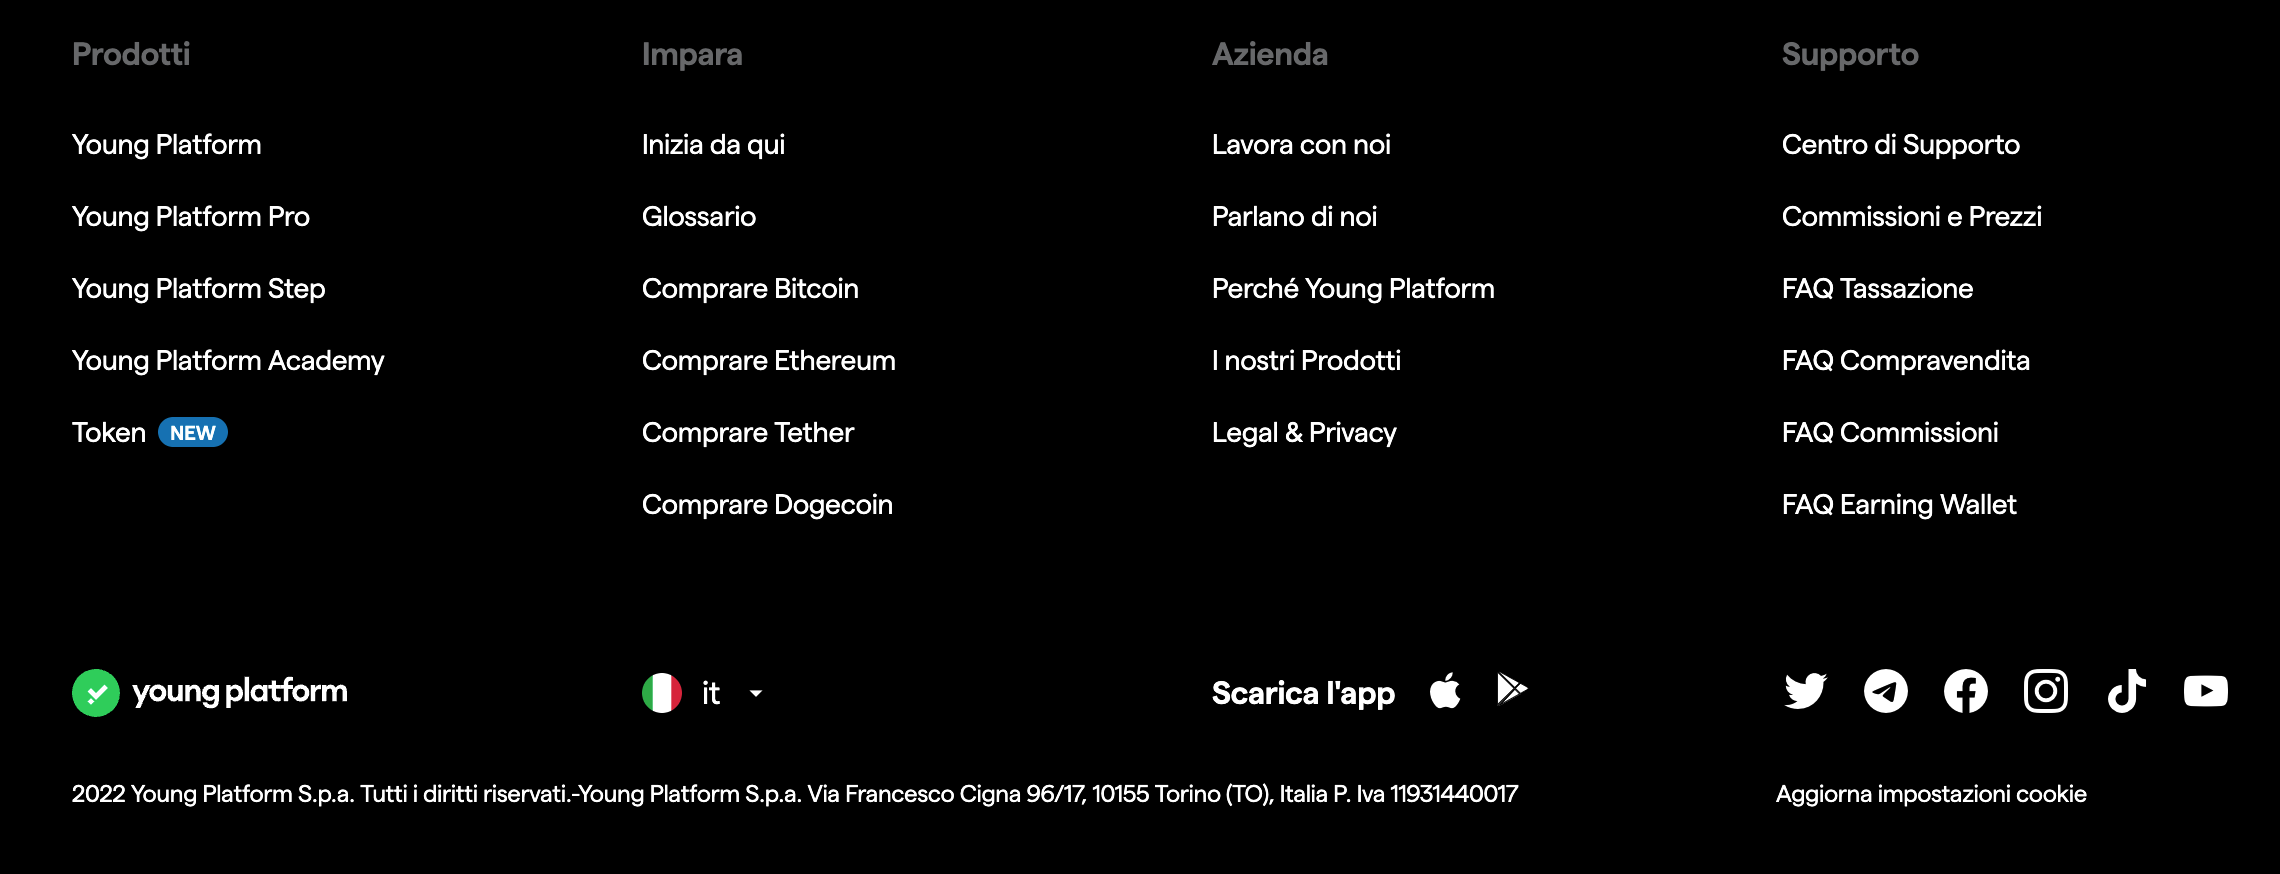
\includegraphics[width=0.80\textwidth]{res/images/footer.png}
	\caption{Footer of the website.}
	\label{fig:footer}
\end{figure}

\subsubsection{What}

\centerline{\textit{What does this site offer?}}
This homepage offers several sections which can be divided into:
\begin{itemize}
  \item \textit{Introduction}: the user can immediately see a slogan, the 
  sector on which the company focuses and the products (of applications for 
  mobile devices, fig. \ref{fig:homepage-1});

  \item \textit{Introduction to the world of cryptocurrencies}: this 
  section, placed shortly after the previous one just described, aims to 
  introduce novice users to this world. The company has collaborated with 
  an important television personality of the 2000s linked to a television 
  program for children. Having put the face of such a person allows a 
  neophyte to reassure himself and that he can be guided by a person who is 
  able to use a simple and clear communication style. I think this section 
  is very important to entice users to continue visiting the site 
  (fig. \ref{fig:introduction-1});

  \begin{figure}[H]
    \centering
    
\includegraphics[width=0.80\textwidth]{res/images/introduction-1.png}
    \caption{Section introducing content for novice users.}
    \label{fig:introduction-1}
  \end{figure}

  \item \textit{Process from registering to use the product}: it briefly 
  illustrates the main steps to be able to use the company's product and to 
  enter the world of cryptocurrencies (fig. \ref{fig:registration-process});

  \begin{figure}[H]
    \centering
    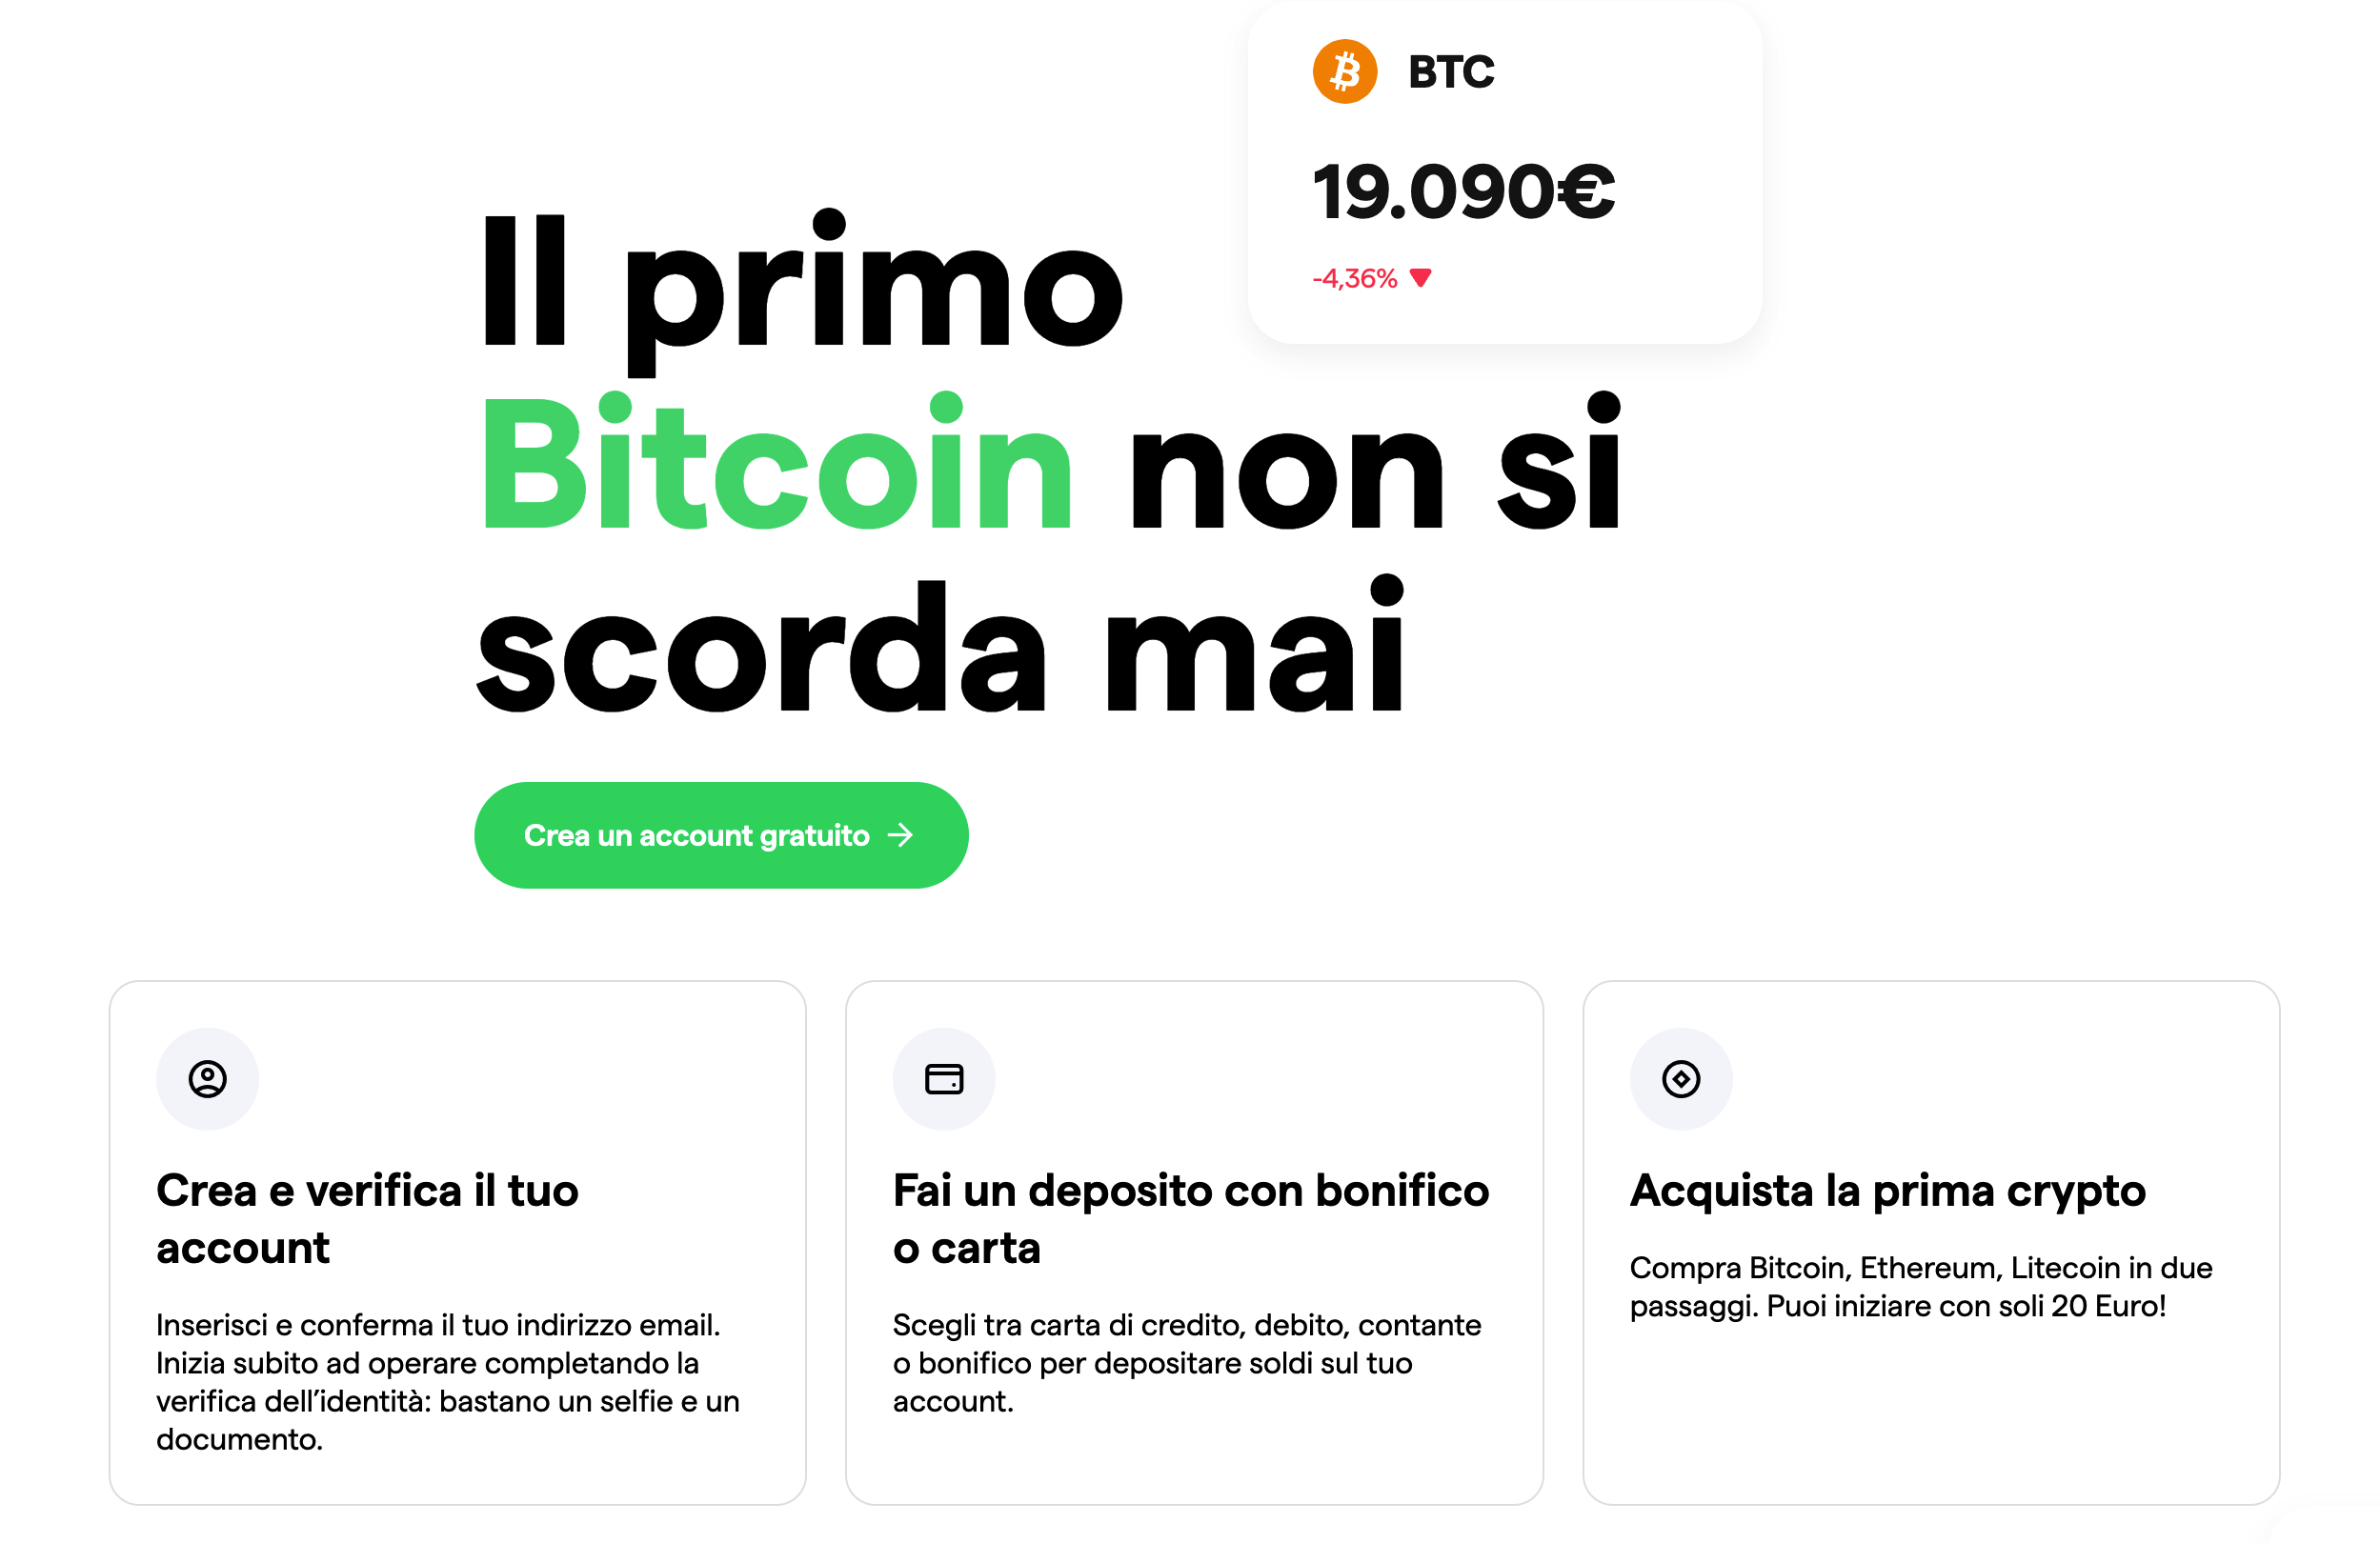
\includegraphics[width=0.80\textwidth]{res/images/registration-process.png}
    \caption{Main steps for using the product offered by the company.}
    \label{fig:registration-process}
  \end{figure}

  \item \textit{Deposit information}: since cryptocurrencies are a field 
  that requires an investment of a certain amount of money from the user, 
  the homepage illustrates a section that reassures the user that it is 
  possible to use different ways to deposit funds in the application 
  (fig. \ref{fig:deposit-options});

  \begin{figure}[H]
    \centering
    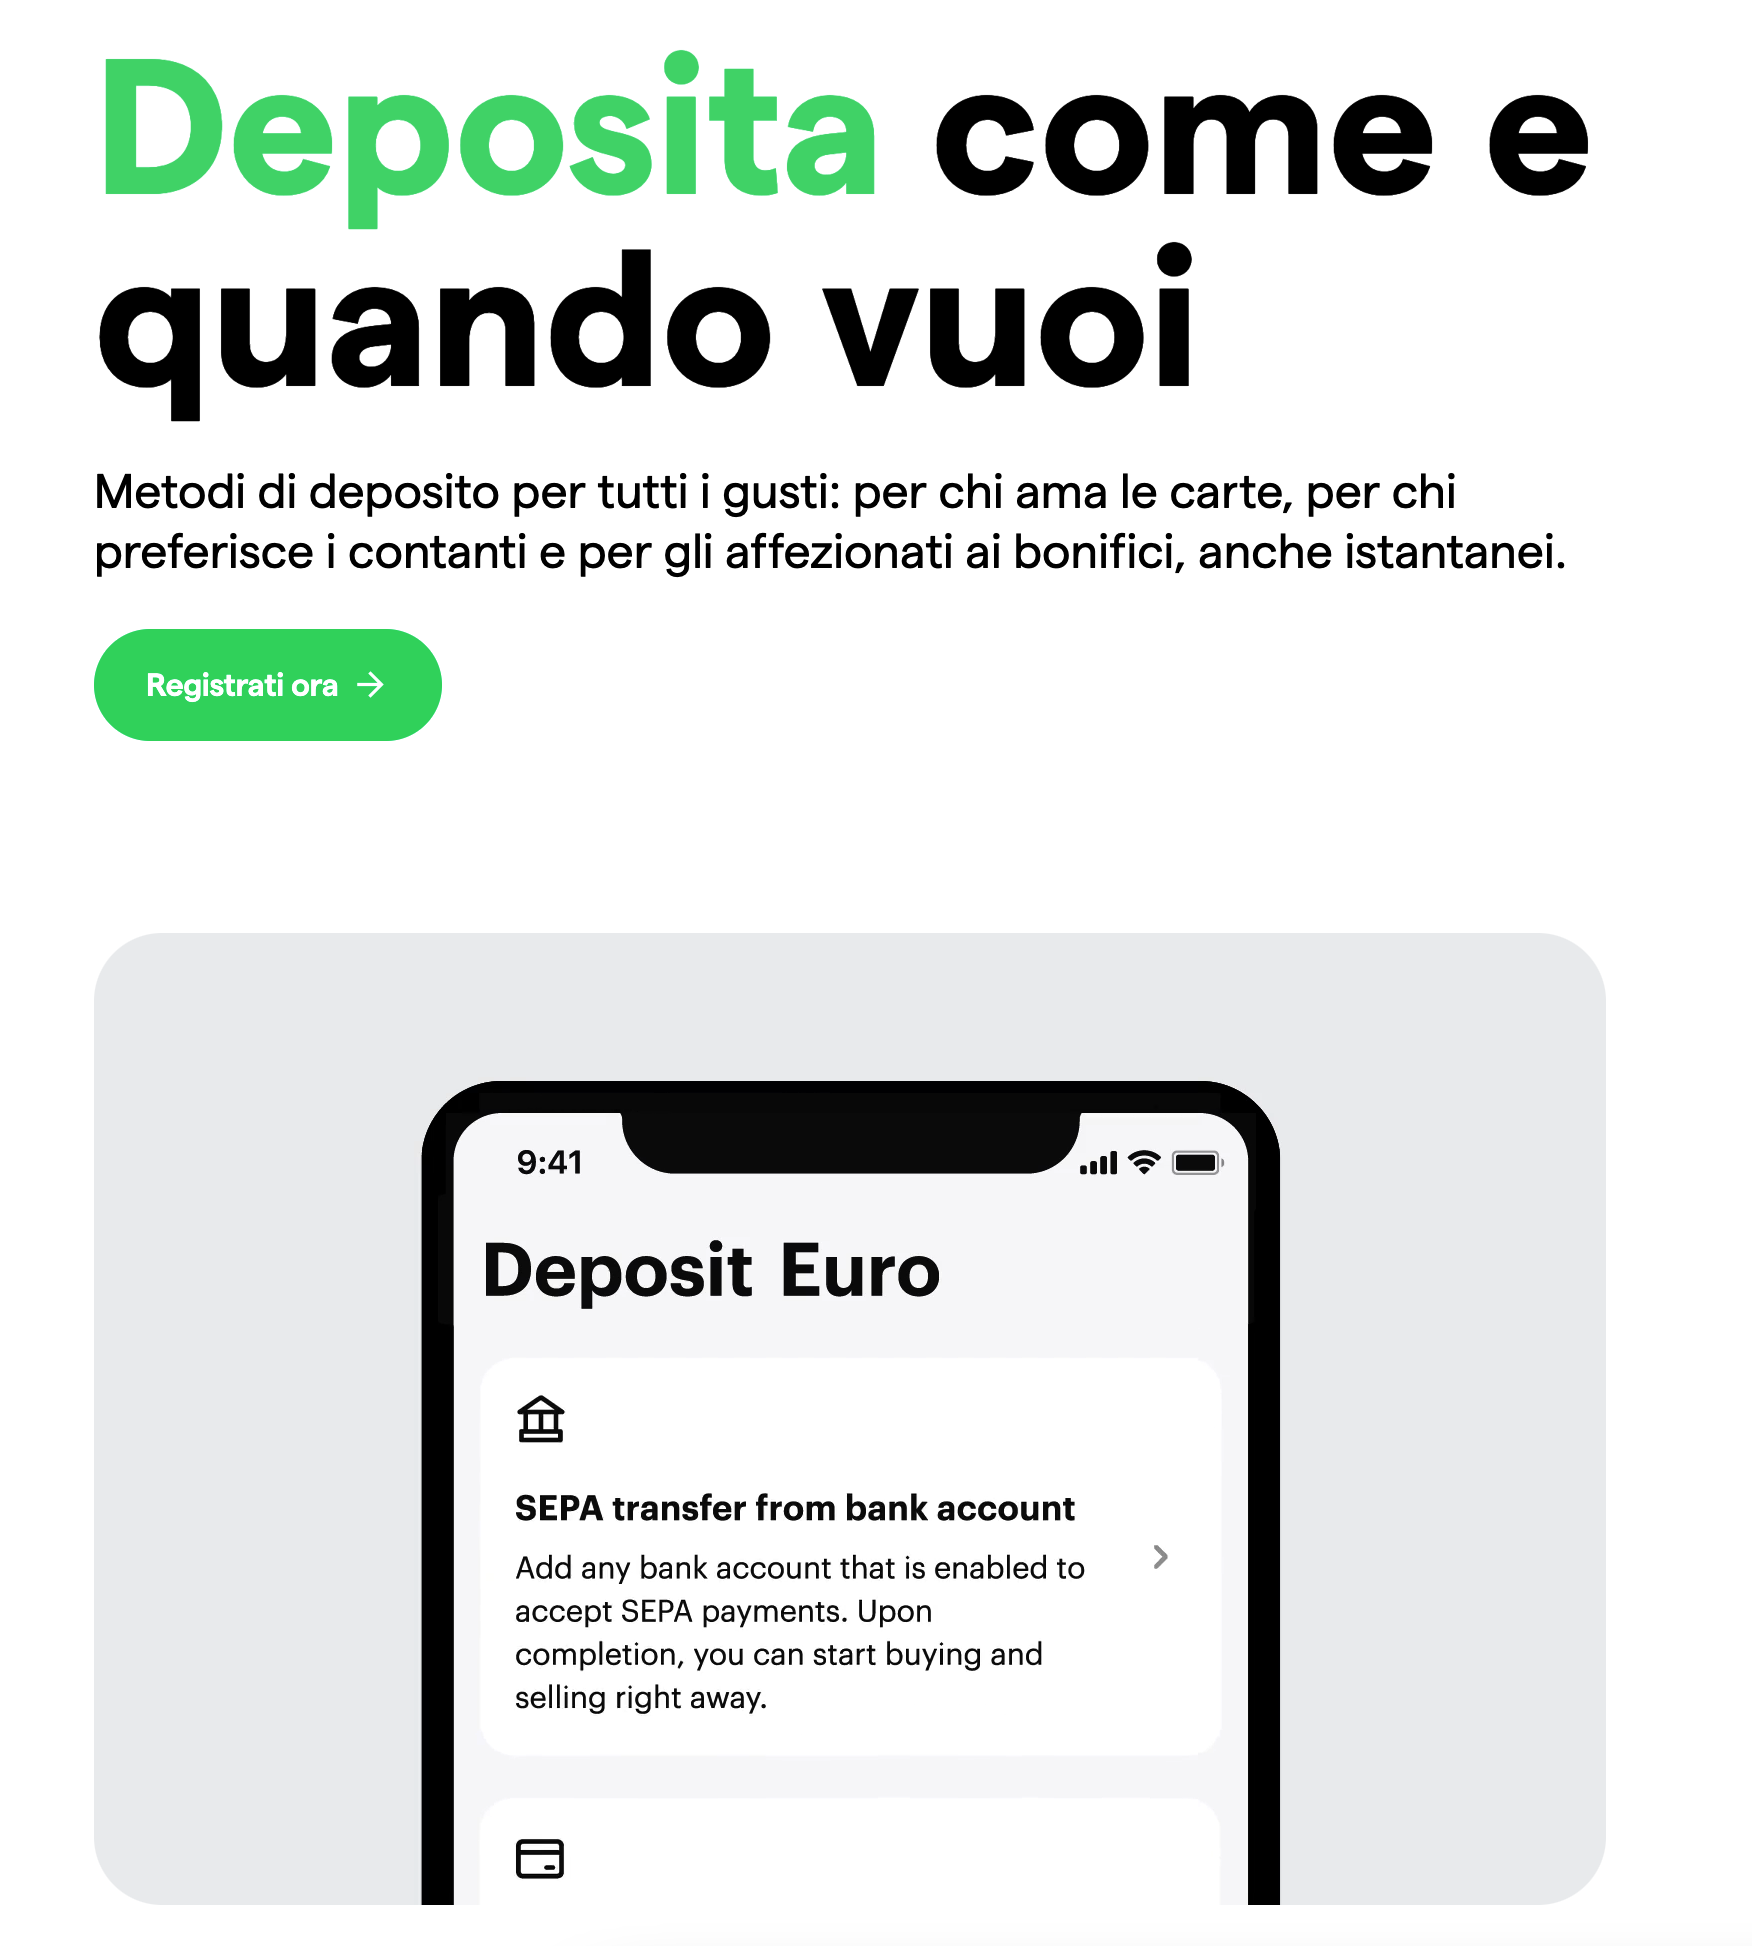
\includegraphics[width=0.50\textwidth]{res/images/deposit-options.png}
    \caption{Information on the types of deposits offered by the product.}
    \label{fig:deposit-options}
  \end{figure}

  \item \textit{Academy, learning articles}: this is another section 
  dedicated to novice users with the aim of reassuring them. In fact, the 
  goal is that the user will be guided step by step, starting from the 
  technological foundations of the blockchain, up to the most advanced 
  concepts of cryptocurrencies. (fig. \ref{fig:academy}).

  \begin{figure}[H]
    \centering
    
\includegraphics[width=0.60\textwidth]{res/images/academy.png}
    \caption{Section introducing articles for learning the fundamentals 
    of the crypto sector.}
    \label{fig:academy}
  \end{figure}
\end{itemize}

\subsubsection{When}

\centerline{\textit{Is the website up to date?}}
When the user reach the homepage for the first time it is not possible 
to tell if the site is up to date. However, one way to verify this is to 
access the \textit{Blog} page, easily accessible from the top main menu. 
From this page it is possible to note that various articles are published 
weekly concerning the latest situations in the cryptocurrency market and 
the innovations introduced in the products offered by the company. For 
each article, the publication date is indicated (fig. \ref{fig:blog}). 
In addition, an estimate of the time to read the article is also 
indicated, so that the user can have a first idea if he can currently 
read a certain article rather than another.

\begin{figure}[H]
	\centering
	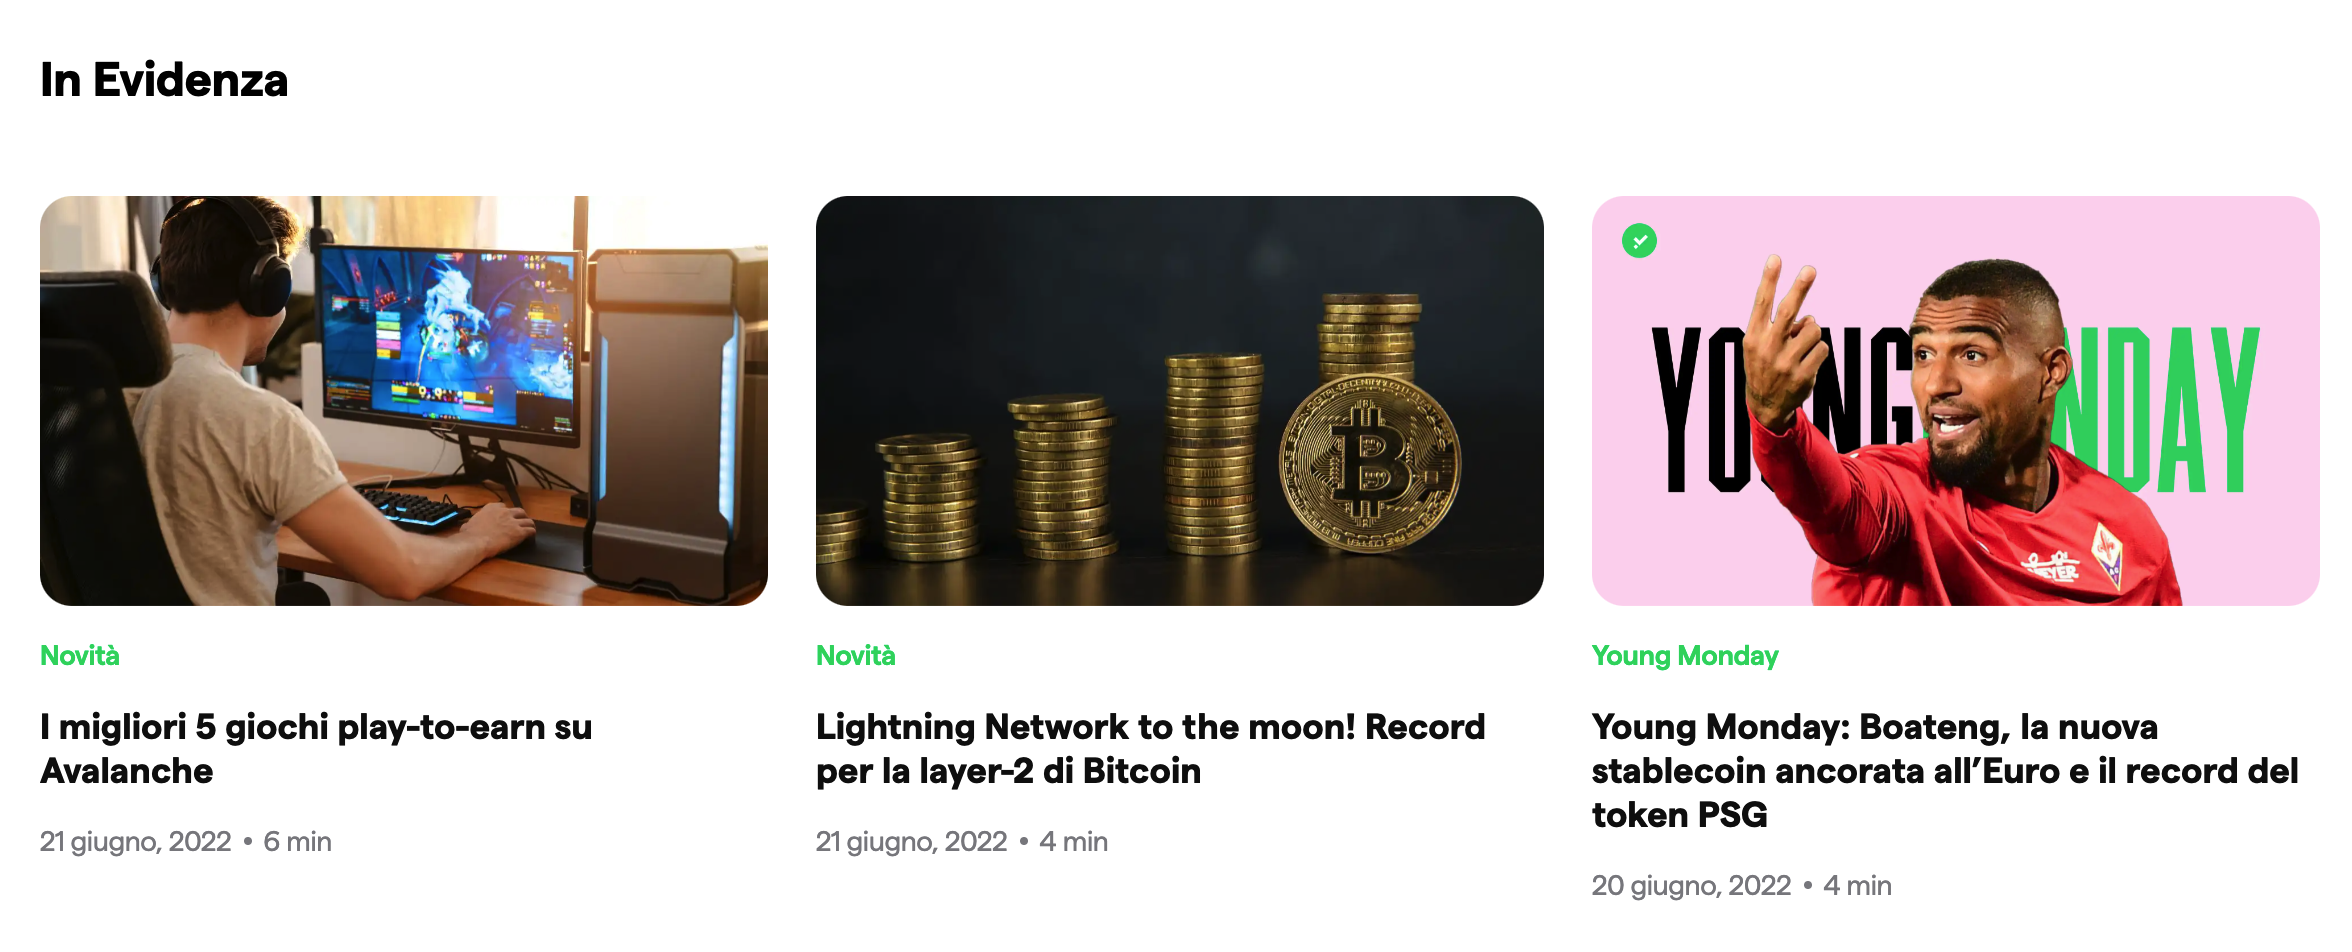
\includegraphics[width=0.90\textwidth]{res/images/blog-1.png}
	\caption{Some blog articles.}
	\label{fig:blog}
\end{figure}

\subsubsection{How}

\centerline{\textit{How can the user achieve what interests him?}}
On the homepage it is possible to reach with a certain simplicity:
\begin{itemize}
  \item where to register and access to use the products;

  \item access content for learning about the world of blockchain and 
  cryptocurrencies;

  \item the blog, a section to stay updated on the latest news closely 
  
  related to the crypto world;

  \item the FAQs;

  \item support, which is very important for this type of product, 
  especially for novice users. Although the company's goal is to make the 
  use of cryptocurrencies usable and accessible, the support represents a 
  very important reference point for the user: cryptocurrencies introduce 
  new knowledge and new dynamics that the user must be familiar with over 
  time. The site, to highlight the importance of this section, has placed 
  the respective item in the main menu, so that the user can reach it very 
  easily and is in a position that is easy to remember 
  (fig. \ref{fig:main-menu}).

  \begin{figure}[H]
    \centering
    
\includegraphics[width=0.90\textwidth]{res/images/main-menu.png}
    \caption{Main homepage menu.}
    \label{fig:main-menu}
  \end{figure}
\end{itemize}

Analyzing the main menu it is possible to notice that it has been placed 
in a clearly visible place. The items are illustrated below:
\begin{itemize}
  \item \textit{Prodotti} (\textit{Products}): when the cursor moves over 
  this item, a submenu appears. Each item in this submenu presents one of 
  the products offered by the company and each item redirects to a specific 
  page;

  \item \textit{Mercati} (\textit{Markets}): this entry redirects to a page 
  that illustrates the trend of the cryptocurrency market;
  
  \item \textit{Token YNG}: this entry redirects to a page that introduces 
  the token created by the company;

  \item \textit{Azienda} (\textit{Company}): when the cursor moves over 
  this item, a submenu appears. Each item in this submenu redirects to a 
  specific page. The items in this submenu are:
  \begin{itemize}
    \item \textit{Ecosistema} (\textit{Ecosystem}): redirects to a page 
    which illustrates the entire ecosystem of products developed by the 
    company;

    \item \textit{Lavora con noi} (\textit{Work with us}): redirects to a 
    page where the company illustrates the values they believe in and a 
    list of job offers;

    \item \textit{Parlano di noi} (\textit{They talk about us}): redirects 
    to a page whose content is partially illustrated in the figure 
    \ref{fig:who-we-are-2};
  \end{itemize}

  \item \textit{Blog}: redirects to a page where all the articles 
  concerning the latest news of the cryptocurrency market are collected;

  \item \textit{Supporto} (\textit{Support}): redirects to a page where 
  the user can contact the company's support if needed.
\end{itemize}

The fact that some items do not redirect to a page but show a drop-down 
submenu makes the site unpredictable from the user's point of view. 
However, this type of submenu is easy to navigate. The submenu of the 
\textit{Azienda} (\textit{Company}) item expands vertically, which is 
preferable to a horizontal expansion. The submenu of the \textit{Prodotti} 
(\textit{Products}) item, on the other hand, expands in a different way: 
the content of the submenu is a two-row and two-column grid. Each entry 
contains the product name, a version of the company logo with a different 
color for each product and a short description of the product. The 
products are divided into two categories: products for 
\textit{cryptocurrency enthusiasts} and \textit{cryptocurrency beginners} 
(fig. \ref{fig:products-submenu}). By doing so, a submenu full of 
information has been created which guides the user towards choosing the 
right product for the user. I think it would have been more useful to swap 
the two columns, in order to give more importance to products dedicated to 
beginners. The fact that the site has used a different color of the 
company logo for each product is very useful for the user, as he can more 
easily recognize one product than the other. A disadvantage of these 
submenus is that they are not \textit{fault tolerant}, that is, as soon as 
the cursor does not point to the item with the submenu, they disappear.
\begin{figure}[H]
  \centering
  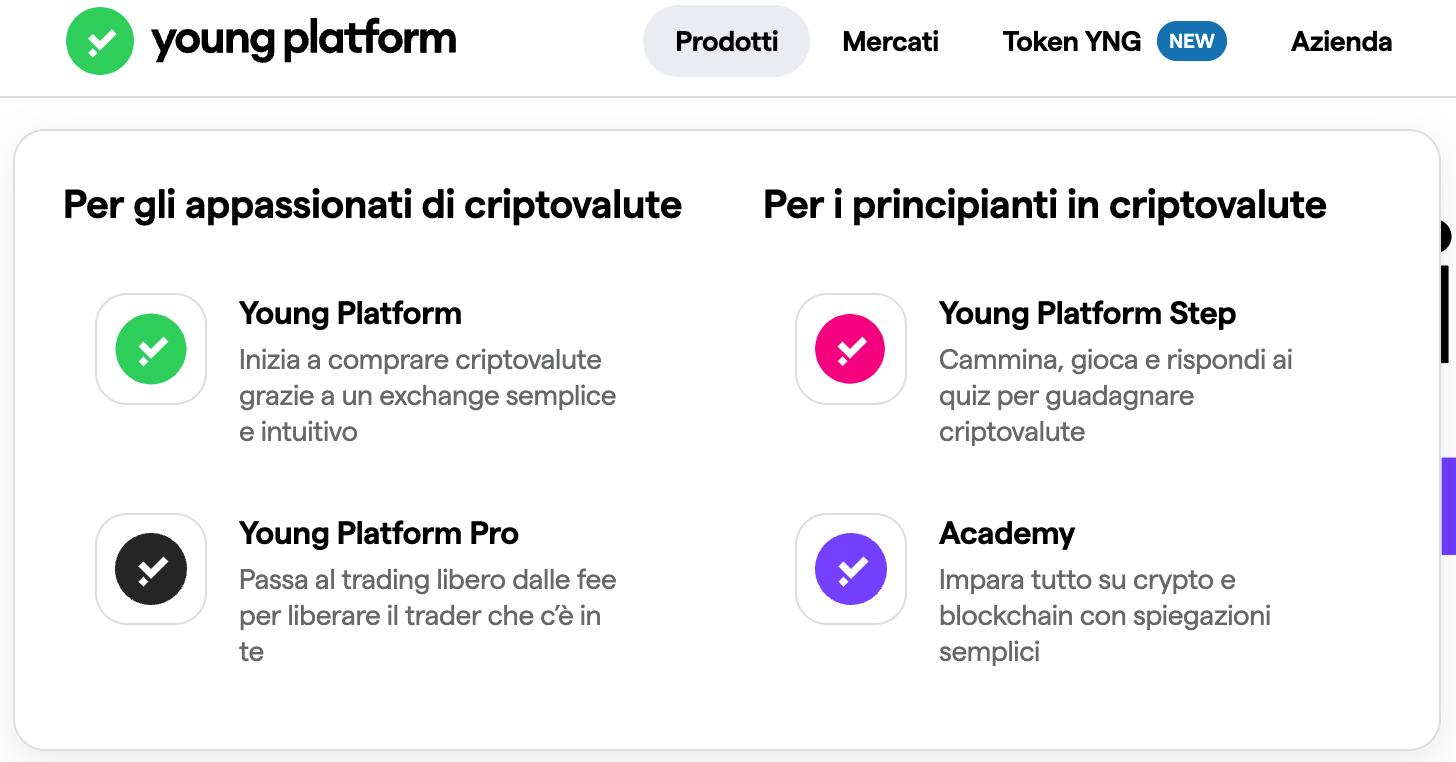
\includegraphics[width=0.70\textwidth]{res/images/products-submenu.png}
  \caption{\textit{Prodotti} (\textit{Products}) item submenu.}
  \label{fig:products-submenu}
\end{figure}